\chapter{Databases}

\index{database}Databases are technically part of the system interface
described in the last chapter, but they are an important application
area in their own right. Different kinds of databases are
appropriate in different situations depending on how much information is to
be stored and what kinds of accesses to the information are supported.
This chapter describes three kinds of databases for which Unicon
provides direct support, enabling you to:

\begin{itemize}
\item Read and write memory-based structures to data files.
\item Use DBM databases as a persistent table data type.
\item Manipulate SQL databases through the ODBC connection mechanism.
\end{itemize}

\section{Language Support for Databases}

Unicon provides transparent access to databases stored in local files
and on remote servers. The term
{\em transparent\/} means that the built-in
functions and operators used to access information in a database are
the same as those used to access information in the memory-based
structures presented in Chapter 2. To do this, connections to databases
are represented by new built-in types that are extensions of the file
and table data types.

Some people might prefer a different syntax for databases from what is
used for data structures. A different syntax, such as one based purely
on function calls, would be consonant with the difference in
performance the programmer can expect to see when accessing data in
files as opposed to memory-based data structures. However, the
performance of operators already depends on the type of the operands.
Consider the expression \texttt{!x}. If \texttt{x} is a structure, its
elements are generated from memory, but if \texttt{x} is a file,
\texttt{!x} reads and generates lines from the file. The goal for
Unicon is to make databases just as easy to learn and use as the rest
of the language, and to minimize the introduction of new concepts.

The word ``database'' means different things to different people; for
some, it is the short form of ``relational database.'' This chapter
uses the term database to refer to any method of providing
{\em persistent structures\/} that store information from one program
run to the next. The operators used to access a database determine
whether one element at a time is read or written, or whether many
operations are buffered and sent to the database together.

\section{Memory-based Databases}

If the entire database fits in memory at once, you can achieve vast
speed-ups by avoiding the disk as much as possible. For example, all
queries to read the database can be performed from memory.  The
database may be modified in memory immediately, and updated on the
disk later on. Memory-based databases are increasingly feasible as
workstation main memories grow larger, they are an excellent choice
for many applications.

One way to implement a memory-based database is to build up your
arbitrary structure in memory, and then use the Icon Program Library
module \texttt{xcodes} to write them out and read them
in. The \index{xcodes}\texttt{xcodes} procedures convert structures
to a string format that can be written to a file, and convert
such strings back into the corresponding structure.
The following sequence saves the
contents of structure \texttt{db} to a file named \texttt{db.dat}.

\iconcode{
db := table() \\
db["Ralph"] := "800-USE-ICON" \\
db["Ray"] := "800-4UN-ICON" \\
dbf := open("db.dat","w") \\
xencode(db, dbf) \\
close(dbf)
}

\noindent
The converse operation, reading in a structure from a file is also
simple:

\iconcode{
dbf := open("db.dat") \\
db := xdecode(dbf) \\
close(dbf) \\
write(db["Ralph"])
}

This approach works great for databases that do not need to be written
to disk on an on-going basis and for which the queries can readily be
expressed as operations on structure types. For example, a telephone
rolodex application would be well-served by this type of database. The
data fits comfortably in memory, updates often occur in batches, and
simple queries (such as a student's name) provide
sufficient access to the data. The other two kinds of databases in this
chapter use traditional database technologies to efficiently address
situations where this type of database is inadequate.

\section{DBM Databases}

A classic database solution on the UNIX platform is provided by the DBM
family of library functions. \index{DBM}DBM stands for Data Base
Manager, and the functions maintain an association between keys and
values on disk, which is very similar to the table data type. DBM was
eventually followed by compatible superset libraries called NDBM (New
Data Base Manager) and GDBM (GNU Data Base Manager). Unicon uses GDBM
on all platforms.

DBM databases are accessed via the \texttt{open()} function using mode
\texttt{"d"} to open a database for reading and writing, or mode
\texttt{"dr"} for read-only access. Once opened, DBM databases
resemble the table data type and are manipulated using table
operations. For example, if \texttt{d} is a DBM file,
\texttt{d[s]}\index{subscript operator} performs a database
insert/update or lookup, depending on whether the expression is
assigned a new value, or \index{dereference}dereferenced for its
current value. Values can also be
inserted into the database with \index{insert()!DBM
database}\texttt{insert(d, k, v)} and read from it with
\index{fetch()!DBM database}\texttt{fetch(d, k)}. \index{delete()!DBM
database}\texttt{delete(d, k)} similarly deletes key \texttt{k} from
the database. DBM databases are closed using the \texttt{close()}
function. The following example program takes a database and a key on
the command line, and writes out the value corresponding to that key.

\iconcode{
procedure main(args) \\
\>   d := open(args[1], "d") {\textbar} stop("can't open ", args[1]) \\
\>   write(d[args[2]]) \\
end
}

If you are wondering why the call to \texttt{open()}
isn't followed by a call to \texttt{close()}, you are
right, it is proper to close files explicitly, although the system
closes all files when the program terminates. How would you generalize
this program to accept a third command-line argument, and insert the
third argument (if it is present) into the database with the key given
by the second argument? You might easily wind up with something like
this:

\iconcode{
procedure main(args) \\
\>   d := open(args[1], "d") {\textbar} stop("can't open ", args[1]) \\
\>   d[args[2]] := args[3] \\
\>   write(d[args[2]]) \\
\>   close(d) \\
end
}

DBM databases are good for managing data sets with a simple
organization, when the size of the database requires that you update
the database a record at a time, instead of writing the entire data
set. For example, if you wrote a Web browser, you might use a DBM
database to store the user's set of bookmarks to Web
pages of interest.

There is one basic limitation of DBM databases when compared with the
table data type that you should know about. DBM databases are
string-based. The keys and values you put in a DBM database get
converted and written out as strings. This makes the semantics of DBM
databases slightly different from tables. For example, a table can have
two separate keys for the integer \texttt{1} and the string
\texttt{"1"}, but a DBM database will treat
both keys as the string \texttt{"1"}. This
limitation on DBM databases also means that you cannot use structure
types such as lists as keys or values in the database. If the type is
not convertible to string, it won't work. You can use
the functions \texttt{xencode()} and \texttt{xdecode()}, described in
the previous section, to manually convert between strings and
structures for storage in a DBM database if you really need this
capability.

\section[SQL Databases]{SQL Databases}

\index{SQL}DBM is great for data that is organized around a single
key, but it is inadequate for complex databases. The industry
standard choice for enterprise-level data organization is the
Structured Query Language (SQL). SQL is supported by every major
database vendor.

Unlike DBM, a SQL database can contain
multiple tables, and those tables are accessed by walking through a set
of results to a query, rather than by accessing individual elements
directly. SQL is designed for industrial-strength relational databases.

\subsection*{The SQL language}

The SQL language was invented by IBM and based on relational database
theory developed by E.F. Codd. A database is a collection of
\textit{tables}, and each table is a collection of \textit{rows}. The
rows in a table contain information of various types in a set of named
\textit{columns}. Rows and columns are similar to records and fields,
except that they are logical structures and do not describe physical
form or layout of the data. There is an ANSI standard definition of
SQL, but many vendors provide extensions, and most vendors are also
missing features from the ANSI standard. Unicon allows you to send any
string you want to the database server, so you can write portable
``vanilla SQL'' or you can write vendor-specific SQL as needed.

SQL was originally intended for text-based interactive sessions between
humans and their databases. Nowadays, SQL is primarily used
``under the covers'' by database
applications that accommodate novice users with
a graphical interface that does not require any knowledge of SQL, while
supporting a SQL ``escape hatch'' for
advanced users who may wish to do custom queries. This duality is
paralleled in the Unicon language by the fact that
Unicon's built-in database operators and functions
duplicate a subset of the capabilities of SQL. There are two ways to do
things: using Unicon operations or using SQL statements.

SQL statements can be divided into several categories, the most
prominent of which are data definition and data manipulation. When
using SQL within a Unicon program, you build up string values
containing SQL statements. In the following examples, the SQL is given
unadorned by double quotes or other Unicon artifacts.

New tables are created with a \texttt{CREATE TABLE} statement, such as

\iconcode{
create table addresses (name varchar(40), address varchar(40),\\
\>\>\>\> phone varchar(15))}

Tables have a primary key that must be unique among rows in the table.
By default the primary key is the first one listed, so \texttt{name} is
the primary key in table \texttt{addresses} above.

SQL's data manipulation operations include
\texttt{SELECT}, \texttt{INSERT}, \texttt{UPDATE}, and \texttt{DELETE}.
\texttt{SELECT} determines the data set being operated on,
picking rows and columns that form some projection of the original
table. \texttt{SELECT} also allows you to combine
information from multiple tables using relational algebra operations.
Most databases are long-lived and evolve to include more columns of
information over time. SQL's ability to select and
operate on projections is an important feature, since code that works
with a certain set of columns continues to work after the database is
modified to include additional columns.

\texttt{INSERT}, \texttt{UPDATE}, and \texttt{DELETE} all modify the
table's contents. \texttt{INSERT} adds new rows to a
table. For example:

\iconcode{
insert into addresses (name, address, phone) \\
\>   \ \ \ \ values ('Nick K',
'1 Evil Empire',
'(123)456-7890') \\
insert into addresses (name, address, phone) \\
\>   \ \ \ \ values ('Vic T',
'23 Frozen Glade',
'(900)888-8888')
}

\texttt{UPDATE} and \texttt{DELETE} can modify or remove sets of rows
that match a particular criterion, as in

\iconcode{
update addresses set address = '666 RTH, Issaquah' \\
\>   \ \ \ \ \ \ \ \ \ \ \ \ \ \ where name = 'Nick K' \\
delete from addresses where name = 'Vic T'
}

This section presented only a few aspects of the SQL language. For
simple database tasks you can in fact ignore SQL and use the Unicon
facilities described in the rest of this chapter. However, for more
complex operations the best solution is to formulate some SQL commands
to solve the problem. A full discussion of SQL is beyond the scope of
this book. For more information on this topic you might want to read
one of the following books: Ramez Elmasri and Shamkant
Navanthe's \textit{Fundamentals of Database Systems,}
C.J. Date and Hugh Darwen's \textit{A Guide to the SQL Standard}.

\subsection*{Database architectures and ODBC}

\index{ODBC}SQL databases are accessed through an underlying Open
DataBase Connectivity (ODBC) transport mechanism. This mechanism allows
the programmer to ignore the underlying architecture. Hiding this
complexity from application programmers is important. The database
architecture may vary from a single process accessing a local database,
to client/server processes, to three or more tiers spanning multiple
networks. Figure 6-1 illustrates the role played by ODBC in providing
Unicon with database access in one- and two-tier configurations. While
this chapter cannot present a complete guide to the construction of
database systems, it provides concrete examples of writing Unicon
client programs that access typical database servers.

\begin{center}
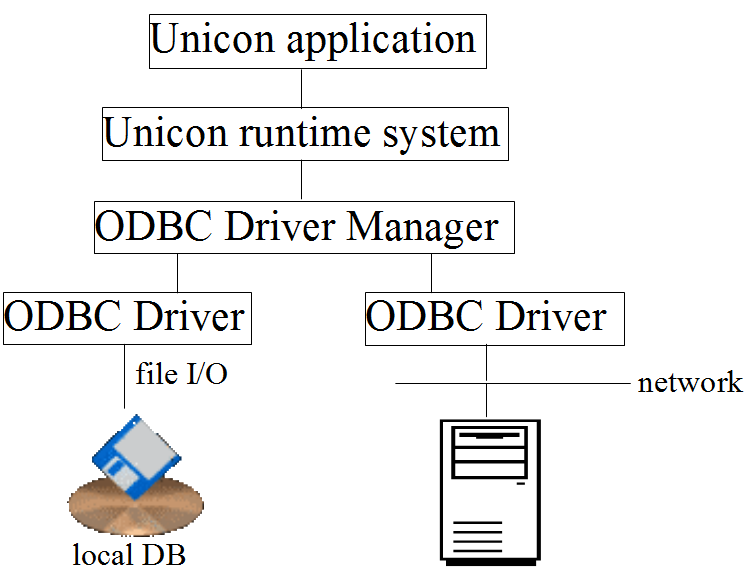
\includegraphics[width=3.2in,height=2.4in]{ub-img/odbcarch.png}
\end{center}

{\sffamily\bfseries Figure 6-1:}
{\sffamily Unicon and ODBC hide underlying architecture from
 applications}

\bigskip

To use Unicon's SQL facilities, you must have several
software components in place. First, you need a SQL database server that
supports ODBC. You can buy a commercial SQL server, or
use a free server such as \index{MySQL}MySQL
(\texttt{www.mysql.com}) or \index{PostgreSQL}PostgreSQL
(\texttt{www.postgresql.org}).

Second, you need an account, password, and permissions on the SQL
server in order to connect to it. The details are
server-dependent and outside the scope of this book.

Third, your client machine needs an \index{driver manager!ODBC}ODBC
driver manager, and an ODBC driver for your SQL server; these must
be configured properly. The driver manager is a component
that connects applications to various databases; ODBC
drivers are dynamic link libraries that database vendors supply
to talk to their database.  Figure 6-2 shows database configuration
for MySQL via the MyODBC GUI dialog box on Windows (left), and in a
{\raise.17ex\hbox{$\scriptstyle\sim$}}/odbc.ini file on Linux (right).
In both cases, configuration involves knowing the internet server
name or IP address, the port, and the database to connect to. For that
triplet, you get to define a name called a DSN or data source name,
which is the name that Unicon will pass in to \texttt{open()}. In the
Windows dialog, this name is a textfield explicitly named as a DSN,
while in the Linux odbc.ini file, it is at the top, inside the square
brackets.

In both cases, there are a lot of additional options which are beyond
the scope of this book.  On Windows, each ODBC driver may have its own
custom dialogs for configuration, while on Linux the odbc.ini file is
more the property of the driver manager and is used to configure all
the various drivers. As a fair warning, the details required in the
dialogs or the exact syntax of the odbc.ini and its required entries
for a given driver change slightly from time to time and are beyond
the scope of this book.  Consult current ODBC documentation for the
driver manager on your platform and the specific database to which
you are connecting.

\bigskip

\noindent
\begin{tabular}{@{}c@{}}{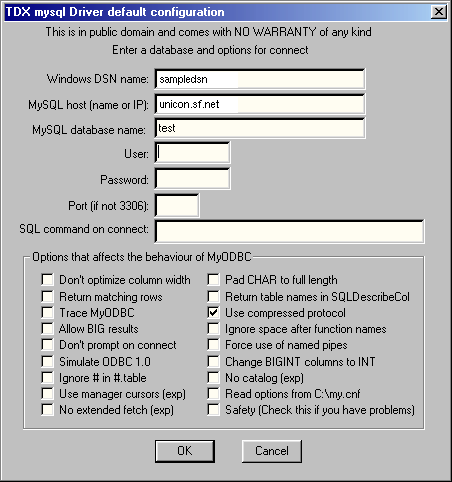
\includegraphics[width=3.8in,height=4.0in]{ub-img/odbcconf.png}}\end{tabular}
\hspace*{.04in}
\begin{tabular}{@{}c@{}}
\begin{tabular}{l}
\texttt{[phones]}\\
\texttt{Driver = /usr/lib64/libmyodbc5.so}\\
\texttt{Description = phone example}\\
\texttt{Server = localhost}\\
\texttt{Database = phonebook}\\
\texttt{Port = 3306}
\end{tabular}
\end{tabular}

{\sffamily\bfseries Figure 6-2:}
{\sffamily Configuring ODBC on Windows (left) and Linux (right)}

\bigskip


Once you have the ODBC software set up,
writing the Unicon client program to connect to your database is
straightforward.

\subsection*{Opening a SQL database}

To connect to a SQL database, call \texttt{open()}
with mode \texttt{"o"}. This establishes a
session with a data source. The filename argument to \texttt{open()} is
the data source to which you are connecting; it is associated with a
particular ODBC driver, remote database server machine or IP number,
and port within the ODBC driver manager. Mode \texttt{"o"} is followed
by additional string arguments to \texttt{open()}. The first is an optional
default table name used in the various functions that take a table
name. Generally the arguments must then include the user name and
password to use in
connecting to the specified data source. Here is an example that
establishes a connection to a database:

\iconcode{
db := open("unicondb", "o", "scott", "tiger")}

The \texttt{open()} function returns a value that supports many of the
operations of both a file and a table, or fails if the connection
cannot be established. The underlying session information is shared by
multiple calls to \texttt{open()} the same database. In addition to
the network connection and SQL session information that is retained,
each database file value maintains a current \textit{selection}
consisting of a set of rows corresponding to the current query, and a
\textit{cursor position} within that selection. When a database is
first opened, the selection consists of a null set containing no rows
and no columns.

\subsection*{Querying and modifying a SQL database}

Subsequent queries to the database can be made by calling
\texttt{sql(db, sqlcmd)}. The \index{sql()}\texttt{sql()} function sets
the current selection within the database and places the cursor at the
beginning of the set of selected rows. For example, to obtain Vic
T's phone number you might say

\iconcode{
sql(db, "select phone from addresses where name='Vic T'")}

Vic's phone number is included if you use the original
\texttt{select *} query, but the more specific your query, the less
time and network bandwidth is wasted sending data that your client
application must filter out. You should do as much work on the server
(in SQL) as possible to make the client more efficient.

Since the function \texttt{sql()} transmits arbitrary SQL statements to
the server, it can be used for many operations besides changing the
current selection. The \texttt{sql()} function returns a null value
when there is no return value from the operation, such as a
\texttt{create table} statement. Its return value can be of varying
type for other kinds of queries, and it can fail, for example if the
SQL string is malformed or requests an impossible operation.

\subsection*{Traversing the selected rows}

To walk through the rows of your current database selection, you call
\index{fetch()!SQL}\texttt{fetch(db)}. The value returned is a
\textit{row} that has many of the operations of a record or a table,
namely field access and subscripting operators. For example, if
\texttt{fetch(db)} returns a row containing columns Name, Address, and
Phone, you can write

\iconcode{
row := fetch(db) \\
write(row.Name) \\
write(row["Address"])
}

\noindent
Called with one argument, \texttt{fetch(db)} advances the cursor
one position. With two arguments, \texttt{fetch(db, col)} produces a
column by name from the current row, without advancing the cursor.
The preceding example could have been written

\iconcode{
   write(fetch(db,"Name")) \\
   write(fetch(db,"Address"))
}

\subsection*{A SQL example application}

\index{SQL}A human resources database might include two tables. One
table might maintain employee information, such as names,
identification numbers, and phone numbers, while another table
maintains entries about specific jobs held, including
employee's ID, the pay rate, a code indicating whether
pay is hourly or salaried, and the job title. Note that the SQL is
embedded within a string literal.

\iconcode{
sql(db, "create table employees (id varchar(11), name
varchar(40),\\
\>\>\>\> phone varchar(15))") \\
sql(db, "create table jobs (id varchar(11), payrate
integer, is\_salaried char,\\
\>\>\>\> title varchar(40))")
}

\noindent
Inserting rows into the database looks like

\iconcode{
sql("insert into employees (id, name, phone) values(32,
'Ray',
'274-2977')")}

Now, how can you print out the job title for any particular employee? If
you have the employee's identification number, the
task is easy, but let's say you just have their name.
These are the kinds of jobs for which SQL was created. Information from
the employees table is effortlessly cross-referenced with the jobs
table by the following SQL. The string is long so it is split into
two lines. A Unicon string literal spans multiple lines when the
closing double quotes has not been found and the line ends with an
underscore character.

\iconcode{
sql(db, "select name,title from employees,jobs \_ \\
\>   \ \ \ \ \ \ where name='Ray' and
employees.id = jobs.id") \\
while write(fetch(db).Title)
}

\subsection*{SQL types and Unicon types}

SQL has many data types, most of which correspond to Unicon types.
\texttt{CHAR} and \texttt{VARCHAR} correspond to Icon
strings; \texttt{INTEGER} and \texttt{SMALLINT} correspond to integers;
\texttt{FLOAT} and \texttt{REAL} correspond to reals, and so on. The
philosophy is to convert between Icon and SQL seamlessly and with
minimal changes to the data format, but you should be aware that these
are not exact matches. For example, it is possible to define a
\texttt{FLOAT} with more precision than an Icon real, and it is easy to
produce an Icon string that is longer than the maximum allowed
\texttt{VARCHAR} size on most SQL servers. Unicon programmers writing
SQL clients must be aware of the limitations of the SQL implementations
they use.

Unicon has structure types for which there is no SQL equivalent. Values
of these types cannot be inserted into a SQL database unless you
explicitly convert them to a SQL-compatible type (usually a string)
using a function such as \texttt{xencode()}.
SQL also has types not found in Unicon such as bit
strings, timestamps, and BLOBS; they are represented
by strings, and strings are used to insert such values into SQL
databases. Strings are also used to represent out-of-range values when
reading SQL columns into Unicon.

\subsection*{More SQL database functions}

SQL databases are feature-rich enough to warrant a suite
of functions in addition to those they
share with other kinds of files and databases. These functions are
described in detail in Appendix A, but some of them deserve special
mention. The function \texttt{dbtables(db)} is useful to obtain a
listing of the data objects available within a particular database.
Function \texttt{dbcolumns(db)} provides detailed information about the
current table that is useful in writing general tools for viewing or
modifying arbitrary SQL databases.

The functions \texttt{dbproduct(db)} and \texttt{dbdriver(db)} produce
information about the DBMS on which \texttt{db} resides, and the
\index{ODBC}ODBC driver software used in the connection.
The function \texttt{dblimits(db)} produces the upper bounds for many
DBMS system parameters, such as the maximum number of columns allowed
in a table. These functions return their results as
a record or list of records whose field names and descriptions
are given in Appendix A.

\section{Tips and Tricks for SQL Database Applications}

In addition to the complexity of learning SQL itself, SQL database
applications have a characteristic flavor which may or may not seem
natural to the Unicon programmer.

\subsection*{Operating on large files}

Asking for 200MB of data in a remote SQL database is a good way to
bring a computer to its knees. Some SQL operations are slow due to an
inefficient query on the remote server, while others are slow because
large amounts of data are transmitted over a limited network
connection. For a fixed amount of data, operation time will vary
radically depending on how it is organized; fewer, larger tuples are
transmitted faster than many smaller tuples.

\subsection*{Use multiple connections to nest queries}

It is common to use more than one table at once. Some times this is
using SQL's \texttt{JOIN} operation, but sometimes it
is not. If you try to nest a second query inside a first one, you will
quickly find that on a given connection, only one \texttt{SELECT} and
one row set is maintained at a time. The second \texttt{SELECT}
replaces the first, so for example:

\iconcode{
db := open("mydsn",
"o", ...) \\
sql(db, {\textquotedblleft}SELECT ...{\textquotedblright}) \\
while r := fetch(db) do \{ \\
\>   sql(db, {\textquotedblleft}SELECT ...{\textquotedblright}) \\
\>   while r2 := fetch(db) do write(r2.foo) \\
\>   \}
}

\noindent
does not work. Within your operating system and database
server's limits, the easy solution is to open multiple
connections to your database:

\iconcode{
db1 := open("mydsn",
"o", ...) \\
db2 := open("mydsn",
"o", ...) \\
sql(db, {\textquotedblleft}SELECT ...{\textquotedblright}) \\
while r := fetch(db) do \{ \\
\>   sql(db2, {\textquotedblleft}SELECT ...{\textquotedblright}) \\
\>   while r2 := fetch(db2) do write(r2.foo) \\
\>   \}
}

\subsection*{Dynamic records}

Rows are represented as a special kind of Unicon record whose
fields are determined at run-time from the names
of selected columns. Record types introduced at runtime
are called \textit{dynamic records}, and they are useful in other
contexts besides databases.

The function \index{constructor!dynamic record
type}\texttt{constructor(rname, field, field, ...)} produces a
procedure that constructs records named
\texttt{rname} with the given fields. The field names
can be arbitrary strings, but only legal identifiers
will be subsequently accessible via the field operator (\texttt{.})

\subsection*{The \texttt{db} library}

The declaration \texttt{link db} provides simplified SQL access routines
for non-SQL programmers.
This library will not allow you to avoid learning SQL for long,
but may ease the conversion from Unicon structure values into SQL
strings for transmission over the network.
The most useful of these procedures is \texttt{dbupdate()}, which sends
a record (tuple) to the database. The following example updates two
columns within a row returned by \texttt{fetch()}.

\iconcode{
row := fetch(db) \\
row.Name := "Bill Snyder" \\
row["Address"] := "6900 Tropicana Blvd" \\
dbupdate(db, row)
}

Of course, before a fetch can be performed, a row set must have been
selected. The procedure \texttt{dbselect(db, columns, filter, order)}
selects tuples containing columns from the database, with optional
filter(s) and ordering rule(s).
Inserting and deleting rows is performed by procedures
\texttt{dbinsert()} and \texttt{dbdelete()}. The \texttt{dbinsert()}
function takes two parameters for each column being inserted, the
column name and then the value.

\subsection*{Unwritable tuples}

Many SQL selections are read-only.  The relational combination of
columns from different tables is powerful, but the resulting
selections are non-updatable.  Another example of a read-only query is
a \texttt{GROUP BY} query, which is usually applied before an
aggregate count. Executing a \texttt{SELECT *} on a single table is
updatable, but if you do something fancier, you will have to know the
semantics of SQL to tell whether the result may be modified.

\section{Summary}

Databases are a standard form of persistent storage for modern
applications. The notation for manipulating a database looks like
a sequence of table and record operations, comprising a
combination of Unicon and SQL statements. Database
facilities give programmers direct access and control over the
information flow to and from permanent storage.
